\documentclass[12pt]{article}

\usepackage[a3paper,landscape]{geometry}

\usepackage[dvipsnames]{xcolor}
\usepackage{lipsum}
\usepackage{lmodern}
\usepackage{enumerate}
\usepackage{amsmath,amssymb}
\usepackage{mathtools}
\usepackage{commath}
\usepackage{upgreek}

\usepackage{commath}
\usepackage[font=small]{caption}
\usepackage[super]{nth}
\usepackage[poster]{tcolorbox}
% \tcbuselibrary{minted} % <- replace by \tcbuselibrary{listings}, if minted does not work for you

% REFERENCES AND OTHERS
\usepackage{aas_macros}
\usepackage{natbib}
\bibpunct{(}{)}{;}{a}{}{,}
\renewcommand{\bibsection}{}

\usepackage{graphicx}
\graphicspath{{figures}}

\usepackage{siunitx}
\sisetup{
    range-phrase=\text{--},
    range-units=single,
    separate-uncertainty=true,
    print-unity-mantissa=false
    }
    \DeclareSIUnit{\parsec}{pc}
    \DeclareSIUnit{\arcsec}{asec}
    \DeclareSIUnit{\erg}{erg}
    \DeclareSIUnit{\arcmin}{arcmin}
    \DeclareSIUnit{\arcsec}{arcsec}
    \DeclareSIUnit{\mas}{mas}
\renewcommand{\figurename}{Fig.}

\tcbuselibrary{listings}
\usepackage{printlen}

\pagestyle{empty}

\usepackage{hyperref}
\hypersetup{
    % bookmarks=true,
    unicode=true,
    pdftoolbar=true,
    pdfmenubar=true,
    pdffitwindow=false,
    pdfstartview={FitH},
    pdftitle={Poster},
    pdfauthor={Tomas Cassanelli},
    pdfcreator={Tomas Cassanelli},
    pdfnewwindow=true,
    colorlinks=true,
    linkcolor=RoyalBlue,
    citecolor=RoyalBlue,
    urlcolor=RoyalBlue
    }

\usepackage{cleveref}

\begin{document}
\begin{tcbposter}[
  coverage={
    spread,
    interior style={
      top color=white,
      bottom color=white
      },
    % watermark text={\LaTeX\ Poster},
    % watermark color=yellow,
    },
  poster={
    % showframe=true,
    columns=4,
    rows=5
    },
  boxes={
    enhanced standard jigsaw,
    sharp corners=downhill,
    arc=2mm,
    boxrule=1mm,
    colback=white,
    opacityback=0.75,
    colframe=black,
    title style={
      left color=black,
      right color=RoyalBlue
      },
    fonttitle=\bfseries\large\scshape
   }
]

\posterbox[
  blankest,
  interior engine=path,
  height=3cm,
  halign=center,
  valign=center,
  fontupper=\bfseries\large,
  colupper=RoyalBlue!25!black,
  underlay={
    \node[right,inner sep=0pt,outer sep=0pt] at (frame.west) {
\includegraphics[height=3cm]{fcfm.pdf}};
    % \node[right,inner sep=0pt,outer sep=0pt] at (frame.west) {\includegraphics[height=3cm]{pink_marble.png}};
    % \node[left,inner sep=0pt,outer sep=0pt] at (frame.east) {\includegraphics[height=3cm]{crinklepaper.png}};
    },
  ]{name=title,column=1,span=3.5,below=top}{
    \resizebox{16cm}{!}{\bfseries Poster title}\\[3mm]
    \href{mailto:tcassanelli@ing.uchile.cl}{tcassanelli@ing.uchile.cl}
  }


\posterbox[adjusted title=References]{
  name=references,
  column=2,
  span=1.5,
  above=bottom}{
    \bibliographystyle{bibstyle_aas}
    \bibliography{poster_template.bib}
  }

\posterbox[adjusted title=Methods, halign=left]{
  name=methods,
  column=2,
  span=2,
  above=references}{

  Here you could describe the methods and a potential cool figure that you may have. Otherwise you could try to make your own using Ti\textit{k}z.

  Ti\textit{k}Z  (PGF plots) is a powerful tool to create in-line-figures in \LaTeX. Unfortunately the learning curve is very steep, but it is definitely worth learning it! There are several online examples that you can browse and edit. Making your own figures will always have an extra value in your report and it is highly appreciated. Source to learn how to make figures are:
  \begin{itemize}
      \item The Ti\textit{k}Z package manual, it is long and sometimes misleading but if you want to master Ti\textit{k}Z is the right place to start!
      \item \url{https://www.ctan.org/pkg/pgf}
      \item Several cool examples: \url{http://www.texample.net/}.
      \item Brief introduction: \url{https://www.sharelatex.com/learn/TikZ_package}
  \end{itemize}

  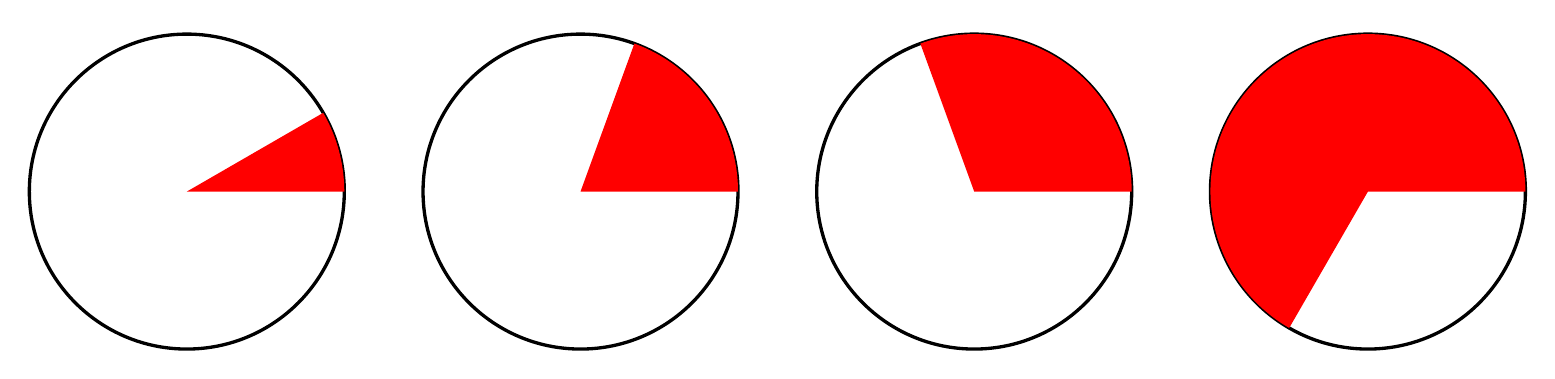
\begin{tikzpicture}[very thick,radius=2cm]
    \begin{scope}
      \path[draw=black,fill=white] (0,0) circle;
      \path[fill=red] (0,0) -- (2,0) arc [start angle=0, end angle=30];
    \end{scope}
    \begin{scope}[xshift=5cm]
      \path[draw=black,fill=white] (0,0) circle;
      \path[fill=red] (0,0) -- (2,0) arc [start angle=0, end angle=70];
    \end{scope}
    \begin{scope}[xshift=10cm]
      \path[draw=black,fill=white] (0,0) circle;
      \path[fill=red] (0,0) -- (2,0) arc [start angle=0, end angle=110];
    \end{scope}
    \begin{scope}[xshift=15cm]
      \path[draw=black,fill=white] (0,0) circle;
      \path[fill=red] (0,0) -- (2,0) arc [start angle=0, end angle=240];
    \end{scope}
  \end{tikzpicture}
  }


\posterbox[adjusted title=Introduction]{
  name=introduction,
  sequence=1 between title and bottom then 2 between title and methods
  }{

  Wecome to the poster tutorial in \LaTeX! The idea of this tutorial is to show you what are the best tools available to create a nice, scientifically and professional poster. Along these blocks I will be suggesting multiple things, these are for figures, references/citations and equations with units.

  We will be using the \texttt{posterbox} environment (part of the \texttt{tcolorbox}), which let's you add block, but be careful because it is easy to \textit{break} the setup. You can change the key \texttt{adjusted title=Introduction} to change the title of this block, but do not change \texttt{name=introduction} otherwise you could break the entire setup. In general, I do not recommend changing much of the style, unless you really know what you're doing! For more I suggest reviewing the official documentation of \href{https://www.ctan.org/pkg/tcolorbox}{\texttt{tcolorbox}}.

  I recommend using the \texttt{siunitx} package, to properly write units and numbers in \LaTeX, makes life so much easier (and professional), an example of this would be:
  \begin{equation}
      I_\nu\del{\nu,\widehat{\mathbf{n}}, \mathbf{r}, t}\dif\nu\dif\Omega \, \unit{\watt\per\m\squared}.
      \label{eq:specific_intensity}
  \end{equation}
  In \cref{eq:specific_intensity} we have added the units in math mode, they also work on text mode, e.g., \unit{\watt\per\m\squared}.

  For more about the units see the online documentation \href{https://ctan.org/pkg/siunitx}{\texttt{siunitsx}}.

  Notice that I have also used the command \texttt{cref} which sets the name of the variable automatically. This is particularly useful when you repeat names like equation, eq., Equation, Eq., not super needed in a poster but another nice tool to have available. You can check the documentation for this in \href{https://ctan.org/pkg/cleveref}{\texttt{cleveref}}.



  \vspace{.5cm}
  The following text it is just to fill in the poster: \lipsum[3]
  }

\posterbox[
  adjusted title=Context,
  % interior style={fill overzoom image=blueshade.png}
  ]{name=context,column=3, between=title and methods}{

  To add a citation we use the \textit{natbib} package, which is the standard way of citation in natural sciences, a citation example would be like this \citep{2022A&A...663A.106C}.
  \noindent The in-line citations are: \citep{2022A&A...663A.106C}, \citet{2022A&A...663A.106C}, \citep[see][]{2022A&A...663A.106C}.

  What I like about natbib is that you can make sentences citing the article. For example: the developed packed by the authors \citet{2022A&A...663A.106C} is capable of run multiple data sets at a time. You can also do \citeauthor{2022A&A...663A.106C} or \citeyear{2022A&A...663A.106C} (see the command in the \texttt{.tex} file, than this will make sense).
  }

\posterbox[
  adjusted title=Conclusions,
  % fit,
  % fit basedim=12pt
  ]{name=conclusions,column*=4,span=1.5,between=methods and bottom}{
  
  You can write your very brief conclusions here!

  }
  
\posterbox[
  adjusted title=Resuts,
  % interior style={fill overzoom image=blueshade.png}
  ]{name=results,column=4, between=top and conclusions}{

  Another figure example using Python. To make figures in Python is pretty easy, just follow the \texttt{sample.py} script that I left in the \texttt{figures/} directory. Notice that I have called the style package which sets the correct \LaTeX-style when making the figure, matching the same font format as in this poster (see \cref{fig:sample}). I you need to know the exact width of the column this is: \uselengthunit{in}\printlength{\textwidth}, in general that shouldn't change much within the same Python script.

  \begin{center}
    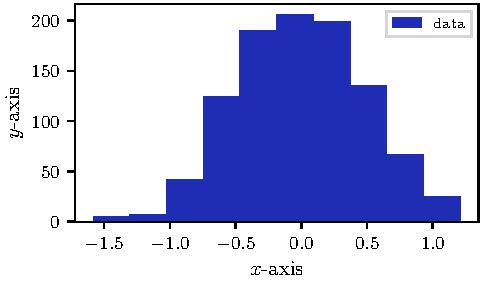
\includegraphics{sample.pdf}
    \captionof{figure}{This is a simple figure made in Python. Notice that the font within the figure matches the poster style. Figure environment will not work in the \texttt{posterbox} command, so remember to use a similar version of this example.}
    \label{fig:sample}
  \end{center}
  

  }



\end{tcbposter}
\end{document}
